\documentclass[11pt,compress,t,notes=noshow, aspectratio=169, xcolor=table]{beamer}

\usepackage{../../style/lmu-lecture}
% Defines macros and environments
% This file is included in slides and exercises

% Rarely used fontstyle for R packages, used only in 
% - forests/slides-forests-benchmark.tex
% - exercises/single-exercises/methods_l_1.Rnw
% - slides/cart/attic/slides_extra_trees.Rnw
\newcommand{\pkg}[1]{{\fontseries{b}\selectfont #1}}

% Spacing helpers, used often (mostly in exercises for \dlz)
\newcommand{\lz}{\vspace{0.5cm}} % vertical space (used often in slides)
\newcommand{\dlz}{\vspace{1cm}}  % double vertical space (used often in exercises, never in slides)
\newcommand{\oneliner}[1] % Oneliner for important statements, used e.g. in iml, algods
{\begin{block}{}\begin{center}\begin{Large}#1\end{Large}\end{center}\end{block}}

% Don't know if this is used or needed, remove?
% textcolor that works in mathmode
% https://tex.stackexchange.com/a/261480
% Used e.g. in forests/slides-forests-bagging.tex
% [...] \textcolor{blue}{\tfrac{1}{M}\sum^M_{m} [...]
% \makeatletter
% \renewcommand*{\@textcolor}[3]{%
%   \protect\leavevmode
%   \begingroup
%     \color#1{#2}#3%
%   \endgroup
% }
% \makeatother


\title{Interpretable Machine Learning}
% \author{LMU}
%\institute{\href{https://compstat-lmu.github.io/lecture_iml/}{compstat-lmu.github.io/lecture\_iml}}
\date{}


\begin{document}

\newcommand{\titlefigure}{figure_man/bike-sharing03.png}
\newcommand{\learninggoals}{
\item See model predictions as a cooperative game
\item Transfer the Shapley value concept from game theory to machine learning
}

\lecturechapter{Shapley Values for Local Explanations}
\lecture{Interpretable Machine Learning}


% \begin{frame}{From Game Theory To Machine Learning}

% \begin{figure}
%     \centering
%     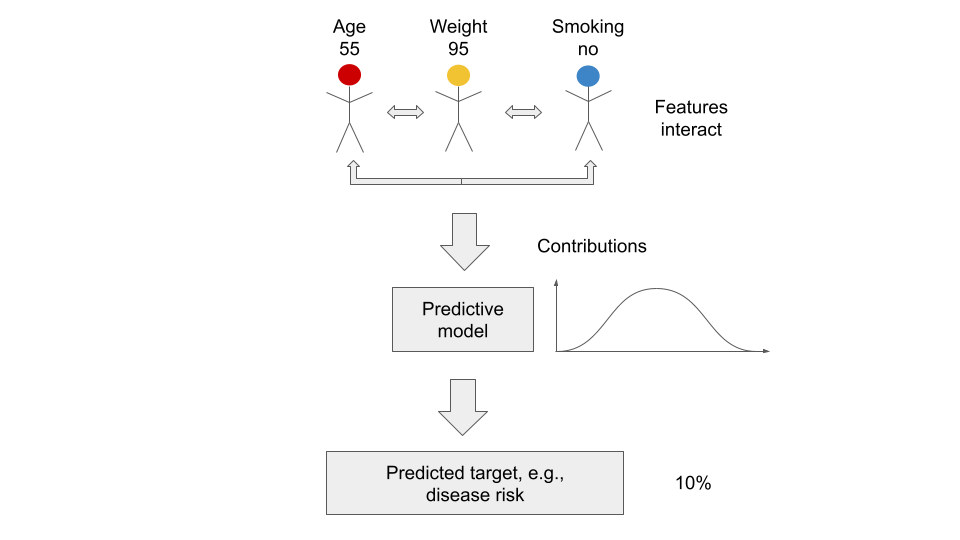
\includegraphics{figure/Shapley_6.png}
% \end{figure}

% \end{frame}

\begin{frame}{From Game Theory to Machine Learning}

\begin{columns}[T,onlytextwidth]
\begin{column}{0.55\textwidth}
\begin{itemize}
  %\item A model prediction is the outcome of multiple features acting together
  %\item How should we attribute this outcome fairly to individual features?
    \item Model prediction depends on feature interactions for a specific observation
  \item \textbf{Goal:} Decompose prediction into \textbf{individual feature contributions}
  \item \textbf{Idea:} Treat features as players jointly producing a prediction
  \item How to fairly assign credit to features?\\
  $\Rightarrow$ Shapley values %provide a principled answer
\end{itemize}
\end{column}

\begin{column}{0.45\textwidth}
  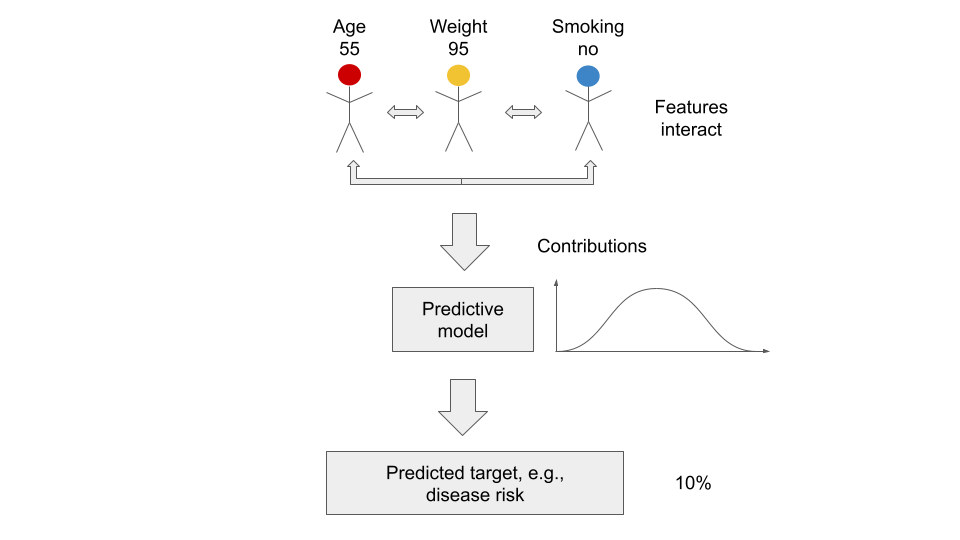
\includegraphics[width=\linewidth, trim=300px 0px 200px 0px, clip]{figure/Shapley_6.png}
\end{column}
\end{columns}

\end{frame}


\begin{frame}{From Game Theory to Machine Learning}
\begin{itemize}%[<+->]
    %\itemsep1em
    \item \textbf{Game:} Predict $\fh(x_1, x_2, \ldots, x_p)$ for a single observation $\xv$
    \item \textbf{Players:} Features $x_j, j \in \pset$, cooperate to produce a prediction
    \item \textbf{Value function:} Defines payout of coalition $S \subseteq P$ for observation $\xv$ by
    
    \medskip
    \centerline{$v(S) = \fh_{S} (\xv_S) - \fh_{\emptyset} , \text{ where }$}
    \medskip
    
    \begin{itemize}
        \item $ \fh_S: \Xspace_S \mapsto \Yspace$ is the PD function 
  $\fh_S(\xv_S) := \int \fh(\xv_S, X_{-S}) \, d\P_{X_{-S}}$\\
    $\leadsto$ "Removes" features in $-S$ by marginalizing, keeping $\fh$ fixed

    \item Mean prediction $\fh_{ \emptyset} := \E_{\xv}(\fh(\xv))$ is subtracted to ensure $v(\emptyset) = 0$
    %$\fh_{S}(\xv_S) := \int_{X_{-S}} \fh(\xv_S, X_{-S})d \P_{X_{-S}}$

    \end{itemize}
    
  \item \textbf{Goal:} 
  Distribute total payout $v(P) = \fh(\xv) - \fh_\emptyset$ fairly among features%Explain how total payout $v(P) = \fh(\xv) - \fh_\emptyset$ is fairly distributed among features %via their average marginal contributions
  \pause
    \item \textbf{Marginal contribution of feature $j$ joining coalition $S$} ($\fh_{ \emptyset}$ cancels):
    
    \medskip
    \centerline{$\Delta(j, S) = v(\Scupj) - v(S) =  \fh_{\Scupj} (\xv_{\Scupj}) - \fh_{S} (\xv_{S})$}
    \medskip
    
    %$\leadsto$ $\E_{\xv}(\fh(\xv))$ cancels out due to the subtraction of value functions
        \item %\textbf{Example:} How features incrementally shift $\fh_S(\xv_S)$ as they join the coalition
         \textbf{Example (3 features):} Feature contributions for joining order $x_1 \rightarrow x_2 \rightarrow x_3$ toward total payout $v(P) = \fh(\xv) - \fh_\emptyset$, each step reflects a marginal contribution
         %\textbf{Example (3 features):} How features incrementally shift $\fh_S(\xv_S)$ from baseline $\fh_\emptyset$ to full prediction $\fh(\xv)$ -- each step reflects a marginal contribution
    %\centerline{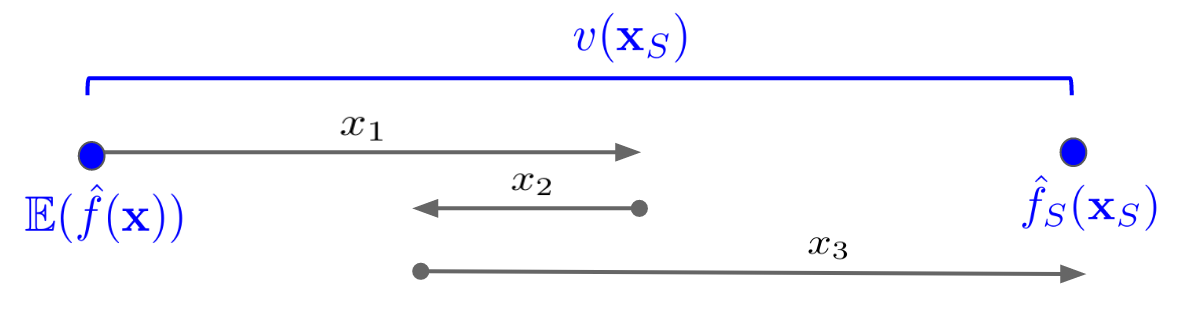
\includegraphics[width=0.5\textwidth, trim=20 0 0 100, clip]{figure_man/shapley_valuefct}}
    \resizebox{\linewidth}{!}{
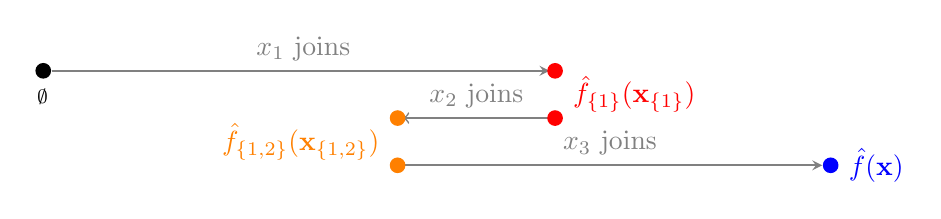
\begin{tikzpicture}[
  dot/.style = {circle, fill, inner sep=2pt},
  arrow/.style = {-stealth, gray, semithick}
]

% --- main nodes --------------------------------------------------------------
\node[dot, black, label={[black]below:$\fh_\emptyset$}]   (start) at (0,0)   {};
\node[dot, blue, label={[blue]right:$\hat f(\mathbf x)$}] (end) at (10,-1.2) {};

% --- x1 ----------------------------------------------------------------------
\draw[arrow, shorten >=2pt] (start) -- (6.5,0) node[midway,above] {$x_1$ joins};
\node[dot, red] at (6.5,0) {};
\node[dot, white, label={[red]right:$\hat f_{\{1\}}(\mathbf x_{\{1\}})$}] at (6.5,-.3) {};

% --- x2 ----------------------------------------------------------------------
\coordinate (x2R) at (6.5,-.6);
\coordinate (x2L) at (4.5,-.6);
\draw[arrow, ->, shorten >=2pt] (x2R) -- (x2L) node[midway,above] {$x_2$ joins};
\node[dot, red]    at (x2R) {};
\node[dot, orange] at (x2L) {};

% --- x3 ----------------------------------------------------------------------
\coordinate (x3L) at (4.5,-1.2);
\draw[arrow] (x3L) -- (end) node[midway,above] {$x_3$ joins};
\node[dot, orange] at (x3L) {};
\node[dot, white, label={[orange]left:$\hat f_{\{1,2\}}(\mathbf x_{\{1,2\}})$}] at (4.5,-.9) {};

\end{tikzpicture}
}

\end{itemize}
\end{frame}
% \begin{frame}{Shapley Values}
%   We can use Shapley values to explain individual predictions $\fh(\xv)$ of a machine learning model $\fh$:
% \begin{itemize}
%   \item Players $\hat{=}$ feature values of $i$-th observation $x_j, j \in \pset$.
%   \item Features cooperate to produce a prediction $\fh(x_1, x_2, \ldots, x_p)$.
%   \item The value function / payout of coalition $S$ for observation $\xv$ is
%     $$v(S) =  \fh_{S} (\xv_S) - \E_{\xv}(\fh(\xv)),$$ 
%     where $\xv_S = \{x_j\}_{j \in S}$ and $\fh_S: \Xspace_S \mapsto \Yspace$.
% \item The marginal prediction $\fh_S$ is defined as $\fh_{S}(\xv_S) := \int_{X_{-S}} \fh(\xv_S, X_{-S})d \P_{X_{-S}}$
% \item We have already seen the marginal prediction in action in the PDP.
% \item The subtraction of $\E_{\xv}(\fh(\xv))$ is necessary so that $v$ is a value function with $v(\emptyset) = 0$.
% \item By using the marginal prediction, we have defined what it means for features to be \enquote{missing} for the prediction: We remove it by integrating over its distribution.
% \end{itemize}
% \begin{center}
% \vspace{-0.3cm}
% 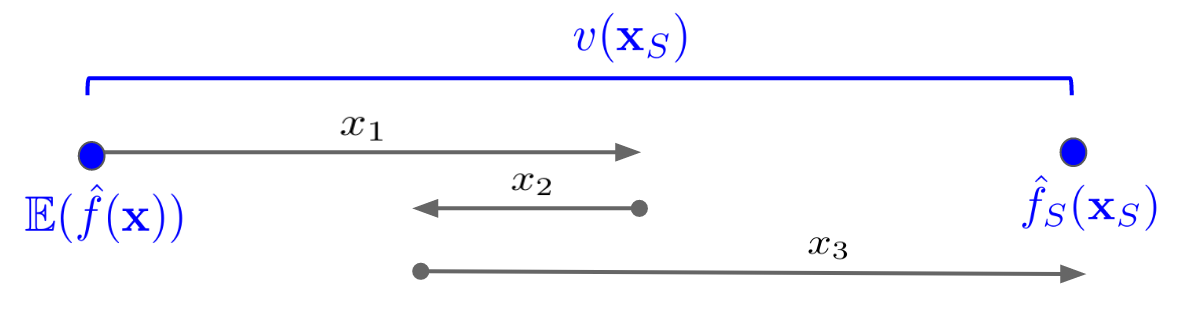
\includegraphics[width=0.6\textwidth]{figure_man/shapley_valuefct}
% \end{center}

% \begin{itemize}
%  \item Shapley values tell us what the payout of each feature is, i.e., how each feature contributes to the overall prediction of a specific observation.
%     \item The Shapley value is the average marginal contribution of a feature towards the prediction \textbf{across all possible feature coalitions}.
%     \item The sum of Shapley values over all features yields the difference between the average prediction of all data points (baseline) and the selected individual prediction.
%   \end{itemize}
% \end{frame}



\begin{frame}{Shapley Value - Definition \citebutton{Shapley (1953)}{https://doi.org/10.7249/P0295} \citebutton{Strumbelj et al. (2014)}{https://doi.org/10.1007/s10115-013-0679-x}}
  %Using the order definition, the Shapley value for feature $j$ and a given observation $\xv$ is computed by:
  %Shapley value $\phi_j$ of feature $j$ for observation $\xv$ via \textbf{order definition}:
  \textbf{Order definition:} Shapley value $\phi_j(\xv)$ quantifies contribution of $x_j$ via

     $$ \phi_j(\xv)  = \frac{1}{|P|!} \sum_{\tau \in \Pi} \underbrace{\fh_{\Stauj}(\xv_{\Stauj}) - \fh_{\Stau}(\xv_{\Stau})}_{\Delta(j, \Stau)~\text{marginal contribution of feature $j$}} $$ %S \subseteq P\setminus \{j\}
     
     
\begin{itemize}
  \item \textbf{Interpretation:}  $\phi_j(\xv)$ quantifies how much feature $x_j$ contributes to the difference between $\fh(\xv)$ and the mean prediction $\fh_\emptyset$

  %$x_j$ contributed $\phi_j$ to difference between $\fh(\xv)$ and mean prediction\\
  $\leadsto$ Marginal contributions and Shapley values can be negative
  %$x_j$ contributed $\phi_j$ to prediction $\fh(\xv)$ compared to average prediction
  % of Shapley value $\phi_j$ for feature $j$ and observation $\xv$:\\
  %Feature value $x_j$ contributed amount $\phi_j$ to prediction $\fh(\xv)$ compared to the average prediction
   \item \textbf{Exact computation of $\phi_j$:} Using PD function 
   %$\fh_{S}(\xv_S) =  \frac{1}{n} \sum_{i=1}^n \fh_S^{(i)}(\xv_S) = \frac{1}{n} \sum_{i=1}^n \fh(\xv_S, \xv_{-S}^{(i)})$ 
   $\fh_{S}(\xv_S) = \frac{1}{n} \sum_{i=1}^n \fh(\xv_S, \xv_{-S}^{(i)})$ 
   yields
   %for any set of features $S$ can be used which yields
   %$$ \phi_j(\xv) = \frac{1}{|P|! \cdot n} \sum_{\tau \in \Pi} \sum_{i = 1}^n \fh_{\Smj}^{(i)}(\xv_{\Smj}) -  \fh_{\Sm }^{(i)}(\xv_{\Sm}) $$
    $$ \phi_j(\xv) = \frac{1}{|P|!} \sum_{\tau \in \Pi} \frac{1}{n} \sum_{i = 1}^n
   \fh(\xv_{\Stauj}, \xv_{\minusStauj}^{(i)}) - \fh(\xv_{\Stau}, \xv_{- \Stau}^{(i)})
   $$
   $\leadsto$ $\fh_S$ marginalizes over all features not in $S$ using all observations $i = 1, \ldots, n$\\
   $\leadsto$ Exact computation requires $|P|! \cdot n$ marginal contribution terms
   
\end{itemize}
\lz
%\tiny
%Shapley, Lloyd S. 1953. $"$A Value for N-Person Games.$"$\\
%\vspace{0.2cm}
%Strumbelj, Erik, Igor Kononenko, Erik Strumbelj, and Igor Kononenko. 2014. $"$Explaining prediction models and individual predictions with feature contributions.$"$

\end{frame}


% \begin{frame}{Estimation: A practical problem}
%   \begin{itemize}[<+->]
%   %\itemsep1em
%       \item Exact Shapley value computation is problematic for high-dimensional feature spaces\\
%       $\leadsto$ For 10 features, there are already $|P|! = 10! \approx 3.6$ million possible orders of features
%       \item Additional problem due to estimation of the marginal prediction $\fh_{\Stau}$: Averaging over the entire data set for each coalition $\Stau$ introduced by $\tau$ can be very expensive for large data sets
%       \item Solution to both problems is sampling:
%       Instead of averaging over $|P|! \cdot n$ terms, we approximate it using a limited amount of $M$ random samples of $\tau$ to build coalitions $\Stau$
%       %We calculate the Shapley value over $M$ samples -- for each sample, we sample one order of features and one data point to replace missing features
%       \item $M$ is a tradeoff between accuracy of the Shapley value and computational costs\\
%       $\leadsto$ The higher $M$, the closer to the exact Shapley values, but the more costly the computation
%       %- the higher $M$, the closer we get to the true Shapley values, but the more costly the computation becomes
%   \end{itemize}
% \end{frame}

\begin{frame}{Estimation: A Practical Problem}
\begin{itemize}[<+->]
  \item \textbf{Exact computation is infeasible for many features:}\\
        For $|P| = 10$, the number of permutations is $10! \approx 3.6$ million\\
        $\leadsto$ Complexity grows factorially with feature count

\item \textbf{Additional challenge: Estimating marginal predictions (PD functions)}\\
Each permutation $\tau$ defines a coalition $\Stau$ needing its own estimate of $\fh_{\Stau}(\xv_{\Stau})$\\
$\leadsto$ With $|P|!$ permutations and $n$ data points, the number of such estimates grows rapidly, making marginalization costly


  \item \textbf{Solution: Sampling-based approximation}\\
        Instead of computing $|P|! \cdot n$ terms, we approximate using $M$ random samples of permutations $\tau$ and data points

  \item \textbf{Tradeoff: Accuracy vs. Efficiency}\\
        Larger $M$ improves Shapley approximation\\
        $\leadsto$ Higher cost, but better fidelity to the exact value
\end{itemize}
\end{frame}


\newcommand{\xk}{\mathbf{x}^{(k)}}

\begin{frame}{Approximation Algorithm \citebutton{Strumbelj et al. (2014)}{https://doi.org/10.1007/s10115-013-0679-x}}
%Estimation of $\phi_j$ for observation $\xv$ of model $\fh$ fitted on data $\D$ using sample size $M$:
Estimate Shapley value $\phi_j$ of observation $\xv$ for feature $j$:

%\vspace{0.25cm}
  \begin{enumerate}[<+->]
  \item[$\bullet$] \textbf{Input:} $\xv$ obs. of interest, $j$ feat. of interest, $\fh$ model, $\D$ data, $M$ iterations
      \item For $m = 1, \ldots, M$ \textbf{do}:
      \begin{enumerate}
        \item Sample random permutation $\tau = (\tau^{(1)}, \ldots, \tau^{(p)}) \in \Pi$ of feature indices% = (\tau^{(1)}, \ldots, \tau^{(p)})
        %\item Select random data point $\xv^{(k)} \in X$.
        %\item Let $\Sm := \Sm$ be the set of features before $j$ of order $\tau$ forming a coalition
        %\item Determine coalition $\Sm := \Stau$, i.e., the set of feat. before feat. $j$ in order $\tau$
        \item Let coalition $\Sm := \Stau$ be the set of features preceding $j$ in $\tau$
        \item Sample random data point {\color{blue} $\mathbf{z}^{(m)} \in \D$} (so-called background data)%\\
        %$\leadsto$ used to marginalize over
        %\item Order feature values in $\xv$ according to $\tau$: $\xv_{\tau} = (x_{\tau^{(1)}}, \ldots, x_{\tau^{(j)}}, \ldots, x_{\tau^{(p)}})$
        %\item Order feature values in $\mathbf{z}^{(m)}$ according to $\tau$: $\mathbf{z}_{\tau}^{(m)} = (z_{\tau^{(1)}}^{(m)}, \ldots, z_{\tau^{(j)}}^{(m)}, \ldots, z_{\tau^{(p)}}^{(m)})$
        % \item Construct two artificial obs. by replacing feature values from $\xv$ with $\mathbf{z}^{(m)}$:
        %   \begin{itemize}
        %   \setlength\itemsep{.5em}
        %     \item % 
        %     $ \xjp  = (\underbrace{x_{\tau^{(1)}}, \ldots, x_{\tau^{(|\Sm|)}}, x_{j}}_{\xv_{\Smj}}, \underbrace{z_{\tau^{(|\Sm|+2)}}^{(m)} , \ldots, z_{\tau^{(p)}}^{(m)}}_{\mathbf{z}^{(m)}_{\minusSmj}} )$
        %     takes features $\Smj$ from $\xv$
        %     %(with value of feature $j$ from $\xv$)
        %     \item % \xjm =
        %     $ \xjm = (\underbrace{x_{\tau^{(1)}}, \ldots, x_{\tau^{(|\Sm|)}}}_{\xv_{\Sm}}, \underbrace{z_{j}^{(m)} , z_{\tau^{(|\Sm|+2)}}^{(m)} , \ldots, z_{\tau^{(p)}}^{(m)}}_{\mathbf{z}^{(m)}_{-\Sm}} )$
        %     takes features $\quad$  $\Sm$ from $\xv$ (takes $\{j\}$ randomly)
        %     %(without value of feature $j$ from $\xv$)
        %   \end{itemize}
        \item Construct two hybrid observations by combining values from $\xv$ and {\color{blue} $\mathbf{z}^{(m)}$}:
\begin{itemize}
\setlength\itemsep{0.5em}
  \item $
  \xjp = (x_{\tau^{(1)}}, \ldots, x_{\tau^{(|\Sm|)}}, x_j, 
          {\color{blue}z_{\tau^{(|\Sm|+2)}}^{(m)}, \ldots, z_{\tau^{(p)}}^{(m)}})
  $\\
  $\leadsto$ includes $\xv_{\Smj}$ (features in $\Sm \cup \{j\}$ from $\xv$), rest from {\color{blue} $\mathbf{z}^{(m)}$}
  
  \item $
  \xjm = (x_{\tau^{(1)}}, \ldots, x_{\tau^{(|\Sm|)}}, 
          {\color{blue}z_j^{(m)}, z_{\tau^{(|\Sm|+2)}}^{(m)}, \ldots, z_{\tau^{(p)}}^{(m)}})
  $\\
   $\leadsto$ includes $\xv_{\Sm}$ (features in $\Sm$ excl. $x_j$ from $\xv$), rest from {\color{blue} $\mathbf{z}^{(m)}$}
\end{itemize}
        \item Compute marginal contribution $\Delta(j, \Sm) = \fh(\xjp) - \fh(\xjm)$ %\\
        %$\leadsto$ $\fh_{\Sm}(\xv_{\Sm})$ is approximated by $\fh(\xv_{-j}^{(m)})$ and  $\fh_{\Smj}(\xv_{\Smj})$ by  $\fh(\xv_{+j}^{(m)})$ over $M$ iters.
        %$\hat =$ A random sample from the marginal contribution of feature $j$ to coalition $\Sm$
        \end{enumerate}
        
    \item Compute Shapley value $\phi_j = \frac{1}{M}\sum_{m=1}^M \Delta(j, \Sm)$ %= \frac{1}{M} \sum_{m = 1}^M   \fh(\xjp ) -  \fh(\xjm ) $
    \item[$\leadsto$] Over $M$ iterations, the PD functions $\fh_{\Sm}(\xv_{\Sm})$ and $\fh_{\Smj}(\xv_{\Smj})$ are approximated by $\fh(\xjm)$ and $\fh(\xjp)$, where features not in the coalition (to be marginalized) are imputed with values from the random data points {\color{blue} $\mathbf{z}^{(m)}$}
  \end{enumerate}
%\pause
%Each $\phi_j^m$ is a random sample from the marginal contribution of feature $j$ for a sampled coalition introduced by $\tau$.
   
   %$$ \phi_j(\xv) = \frac{1}{|P|! \cdot n} \sum_{\tau \in \Pi} \sum_{i = 1}^n  \fh(\xv_{\Smj}, \xv_{\minusSmj}^{(i)}) - \fh(\xv_{\Sm}, \xv_{- \Sm}^{(i)})  $$
   
   % \vspace{0.25cm}
    %\tiny{Strumbelj, Erik, Igor Kononenko, Erik Strumbelj, and Igor Kononenko. 2014. $"$Explaining prediction models and individual predictions with feature contributions.$"$}



\end{frame}

\begin{frame}{Shapley value approximation - Illustration}

\begin{exampleblock}{Definition}
% \[
% \tikzmark{phi}\phi_{\tikzmark{j}j}(%\tikzmark{v}\fh,
% \tikzmark{x}\xv)=\frac{1}{M}\tikzmark{M}\sum_{m=1}^M \left[
% \fh_{\Sm \tikzmark{SJ}\cup j}
% \left(\xv_{\Sm \tikzmark{SJ}\cup j}\right)-
% \fh_{\tikzmark{S}\Sm}\left(\xv_{\tikzmark{S}\Sm}\right)\right]
% \]
$$
\tikzmark{phi}\phi_{\tikzmark{j}j}(%\tikzmark{v}\fh,
\tikzmark{x}\xv)=\frac{1}{M}\tikzmark{M}\sum_{m=1}^M \left[
\fh(\xv_{+j}\tikzmark{SJ}^{(m)}) -
\fh(\xv_{-j}\tikzmark{S}^{(m)})\right]
$$
\begin{tikzpicture}[
  remember picture,
  overlay,
  expl/.style={draw=blue,fill=white,rounded corners,text width=3.7cm},
  arrow/.style={blue,ultra thick,->,>=latex}
]
%%%% Explain Formula I
% \draw<2-3> [draw=white, fill=white, opacity=0]
%       (5.8,0) -- (11,0) -- (11,2) -- (5.8,2) --cycle;
% \node<1>[expl] 
%   (phiex) 
%   at (6,2cm)
%   {Shapley value of feat. $j$};
% \node<2>[expl] 
%   (jex) 
%   at (2,0cm)
%   {for feature $j$};
% \node<3>[expl] 
%   (vex) 
%   at (5,-0.7cm)
%   {$\fh$: pred. function};
\node<1>[expl] 
  (xex) 
  at (4,2cm)
  {$\xv$: obs. of interest};
% \draw<1>[arrow]
%   (phiex.south) to[out=270,in=90] ([xshift= 1ex, yshift=1.5ex]{pic cs:phi});  
% \draw<2>[arrow]
%   (jex.north) to[out=90,in=270] ([yshift=-0.5ex]{pic cs:j});  
% \draw<3>[arrow]
%   (vex.east) to[out=0,in=270] ([xshift= 1ex, yshift=-0.5ex]{pic cs:v});  
\draw<1>[arrow]
  (xex.south) to[out=270,in=90] ([xshift= 0.5ex, yshift=1.5ex]{pic cs:x}); 
  
 %%%% Explain Formula II
% \draw<3-5> [draw=white, fill=white, opacity=0.6]
%       (4,0) -- (6.8,0) -- (6.8,2) -- (4,2) --cycle;
\node<1>[expl] 
  (Sex) 
  at (9,2cm)
  {$\xv$ with feature values in $\xv_{\Sm}$ (other are replaced)};
\node<2>[expl] 
  (Sex) 
  at (5,2cm)
  {Contribution of feature $j$ to coalition $\Sm$};
 \node<1>[expl] 
  (SJex) 
  at (8,-0.8cm)
  {$\xv$ with feature values in $\xv_{\Smj}$};
  \draw<1>[arrow]
  (Sex.south) to[out=270,in=50] ([xshift= 1ex, yshift=2.5ex]{pic cs:S});
 \draw<2>[arrow]
  (Sex.east) to[out=0,in=90] ([xshift= 1ex, yshift=2.5ex]{pic cs:S});
  \draw<1>[arrow]
  (SJex.north) to[out=90,in=270] ([yshift=-1ex]{pic cs:SJ}); 
  \draw<2> [decorate,decoration={brace, amplitude=5pt,mirror,raise=4ex}]  (5.6,1.1) --  (8.85,1.1)
  node[midway,yshift=-3.4em]{\scriptsize $:= \Delta(j, \Sm)$};
  
  \draw<2> [draw=white, fill=white, opacity=0.6]
       (2.5,0) -- (5.5,0) -- (5.5,1.5) -- (2.5,1.5) --cycle;
  %%%% Explain Formula III
  \draw<3> [draw=white, fill=white, opacity=0.6]
       (2.5,0) -- (4.2,0) -- (4.2, 2) -- (2.5,2) --cycle;
  \draw<3> [draw=white, fill=white, opacity=0.6]
        (5.5,0) -- (10.5,0) -- (10.5,2) -- (5.5,2) --cycle;
  \node<3>[expl] 
  (Mex) 
  at (8,2cm)
  {average the contributions of feature $j$};
  \draw<3>[arrow]
  (Mex.west) to[out=180,in=50] ([xshift= 0.5ex, yshift=4ex]{pic cs:M}); 
\end{tikzpicture}
\end{exampleblock}
%\vspace{0.5cm}
\begin{itemize}
    \begin{onlyenv}<1>
    \vspace{50pt}
    % \item The Shapley value assigns a value to each feature $j$ according to the marginal contribution of each player in all possible coalitions
    \end{onlyenv}
    %\invisible<2>{\item The Shapley value assigns a value to each feature $j$ according to the marginal contribution of each player in all possible coalitions}
    %\begin{onlyenv}<3>
    %\item A value function $v(S): 2^{|P|}\mapsto \R$ describes the payout (or gain) achieved by any coalition $\forall S \subseteq P$. The value of the empty coalition must be zero: $v(\emptyset) = 0$.
    %\item The payout of coalition $S$ for observation $\xv$ is 
    %$$v(\xv_S) =  \fh_{S} (\xv_S) - \E (\fh(\xv))$$ 
    %i.e., the difference of the marginal prediction of $\xv_S$ and the average prediction.
    %\end{onlyenv}
    %\begin{onlyenv}<4>
    %\item Example observation from bike sharing data
    %\end{onlyenv}
    % Part II
    %\begin{onlyenv}<5>
    %\item $\Sm$ is a randomly selected set of features: $\Sm \subseteq P \setminus j$ where $P$ denotes the quantity of all features in $X$
    %\item Let $x_{\Sm}$ be a random chosen subset of features in $x_S$ that is hold fix
    %\end{onlyenv}
     %   \begin{onlyenv}<6>
    %\item Let $S_{\lnot m}$ denote the subset of $P$ that is not in $\Sm$.
    %\item Draw the values of all other features $x_{S_{\lnot m}}$ randomly from the set of available values of the regarding feature to calculate $v(x_{\Sm})$
    %\end{onlyenv}
    \begin{onlyenv}<2>
     \item $\Delta(j, \Sm) = \fh(\xjp) -
\fh(\xjm)$ is marginal contribution of feature $j$ to coalition $\Sm$
    \item Here: Feature \textit{year} contributes +700 bike rentals if it joins coalition $\Sm = \{temp, hum\}$ %compared to the expected prediction conditioned on features in coalition $\Sm$ (while other features were taken from a random obs.)
    \end{onlyenv}
    \begin{onlyenv}<3>
    \item Compute marginal contribution of feature $j$ towards the prediction across all randomly drawn feature coalitions $S_1, \ldots , \Sm$
    \item Average all $M$ marginal contributions of feature $j$
    \item Shapley value $\phi_j$ is the payout of feature $j$, i.e., how much feature \textit{year} contributed to the overall prediction in bicycle counts of a specific observation $\xv$
    \end{onlyenv}
\end{itemize}
\vspace*{\fill}
%\vspace*{30pt}
\begin{center}
%\includegraphics<3>[width=0.5\textwidth]{figure_man/shapley_valuefct}
% Link https://docs.google.com/presentation/d/14FZZ4zk7IBZv6XnQA0wDVfCDhmjzf4np5uVj7KrIxXg/edit#slide=id.p
%\includegraphics<4>[page=1, width=1\textwidth]{figure_man/data_shapley}
%\includegraphics<5>[page=2, width=1\textwidth]{figure_man/data_shapley}
%\includegraphics<6>[page=3, width=1\textwidth]{figure_man/data_shapley}
%\includegraphics<7>[page=4, width=1\textwidth]{figure_man/data_shapley}
\includegraphics<1>[page=13, width=1\textwidth]{figure_man/data_shapley}
\includegraphics<2>[page=14, width=1\textwidth]{figure_man/data_shapley}
\includegraphics<3>[page=15, width=1\textwidth]{figure_man/data_shapley}
\end{center}

\end{frame}





% \begin{frame}{Revisited: Axioms for Fair Attributions}
%   We take the general axioms for Shapley Values and apply it to predictions:
%   \vspace{0.25cm}
%   \begin{itemize}[<+->]
%   \itemsep1em
%     \item \textbf{Efficiency}: Shapley values add up to the (centered) prediction: %. 
%     %That means, unlike, e.g., LIME, we get a dense attribution, and not a sparse one.
%     $\sum\nolimits_{j=1}^p\phi_j=\fh(\xv)-\E_{\xv}(\fh(X))$
%     \item \textbf{Symmetry}: If $x_j$, $x_k$ contribute the same, they receive the same payout\\
%     $\leadsto$ interaction effects between features are fairly divided \\
%       $\fh_{S\cup\{j\}}(\xv_{\Scupj}) = \fh_{\Scupk}(\xv_{\Scupk})$ for all $S \subseteq P\setminus\{j,k\}$ then $\phi_j=\phi_k$
%     \item \textbf{Dummy / Null Player}: Shapley value of a feature that does not influence the prediction is zero $\leadsto$ if a feature was not selected by the model (e.g., tree or LASSO), its Shapley value is zero  \\
%       $\fh_{\Scupj}(\xv_{\Scupj})=\fhS(\xv_S)$ for all $S \subseteq P$ then $\phi_j=0$
%     \item \textbf{Additivity}:  For a prediction with combined payouts, the
%       payout is the sum of payouts: $\phi_j(v_1) + \phi_j(v_2)$\\
%       $\leadsto$ Shapley values for model ensembles can be combined
%   \end{itemize}
% \end{frame}

\begin{frame}{Revisited: Axioms for Fair Attributions}
We adapt the classic Shapley axioms to the setting of model predictions:
\vspace{0.25cm}

\begin{itemize}%[<+->]
%\itemsep1em
\item \textbf{Efficiency}: Sum of Shapley values adds up to the centered prediction:
\[
\textstyle\sum_{j=1}^p \phi_j(\xv) = \fh(\xv) - \E_\xv[\fh(\xv)]
\]
$\leadsto$ All predictive contribution is fully distributed among features

\item \textbf{Symmetry}: Identical contributors receive equal value:
\[
\fh_{\Scupj}(\xv_{\Scupj}) = \fh_{\Scupk}(\xv_{\Scupk}) \ \forall S \subseteq P \setminus \{j,k\}
\Rightarrow \phi_j = \phi_k
\]
$\leadsto$ Interaction effects are shared equitably

\item \textbf{Dummy (Null Player)}: Irrelevant features receive zero attribution:
\[
\fh_{\Scupj}(\xv_{\Scupj}) = \fh_S(\xv_S) \ \forall S \subseteq P \Rightarrow \phi_j = 0
\]
$\leadsto$ Shapley value is zero for unused features (e.g., trees or LASSO)

\item \textbf{Additivity}: Attributions are additive across models:
\[
\phi_j(v_1 + v_2) = \phi_j(v_1) + \phi_j(v_2)
\]
$\leadsto$ Enables combining Shapley values for model ensembles

\end{itemize}
\end{frame}



% \begin{frame}{Additional Estimation Trick}


%   The Shapley value can be estimated more efficiently when certain coalitions are always included in the computation, instead of random sampling:
%   \vspace{0.25cm}
%   \begin{itemize}
%   \itemsep1em
%     \item The coalitions with $S = \emptyset$ (i.e., $|S| = 0$) and $S = \{1, \ldots, p\} \setminus j$ have the highest weights in the Shapley value computation $\leadsto$ including them makes Shapley value more stable with fewer samples %Sample weights have to be adapted for the sampled coalitions afterwards.
%     \item Intuition: Adding a feature to the empty coalition gives information about the \textit{pure} first order effect of the feature, which is the effect without any interactions 
%     \item Adding the feature value to the complete set of feature values gives us the information about the total effect of a feature, which is the sum of the main effect and all interaction effects with other features
%     \item For coalition $S = \emptyset$, there are $0! (|P| - 0 - 1)! = 1 \cdot (|P| - 1)! = (p - 1)!$ orders, which is the same for $S = P \setminus \{j\}$: $|P \setminus \{j\}|! (|P| - |P \setminus \{j\}| - 1)! = (p - 1)! (p - (p-1) - 1)! = (p-1)!$
% \end{itemize}
%  \end{frame}

% \begin{frame}{Additional Estimation Trick}
% An example with $p = 5$ features:
% \vspace{0.25cm}
%     \begin{itemize}
%     \itemsep1em
%         \item There are $5! = 120$ orders in total
%         \item In $(5 - 1)! = 24$ orders, we added feature value $x_j$ to the empty set
%         \item In 24 orders, we added the feature value to the otherwise full feature set
%         \item That means with just two sets, we can already get $\frac{48}{120} = 0.4$ of the contributions to the Shapley value
%         \item Similarly, we could proceed with all coalitions of $\{S: |S| = 1\}$ and $\{S: |S| = p - 1\}$
%         \item When some coalitions are added \enquote{manually}, and the rest are sampled, we have to adapt the weights: Let $w$ be the weight of the \enquote{manually} sampled coalitions, $\hat{\phi}_{j,fixed}$ the part of the Shapley value with only the manual contributions and $\hat{\phi}_{j,sample}$ the Shapley value with the sampled coalitions, then the Shapley value is: $w \cdot \hat{\phi}_{j,fixed} + (1 - w) \hat{\phi}_{j,sample}$
%   \end{itemize}
% \end{frame}

% \begin{frame}{Additional Estimation Trick}
%       \begin{center}
%         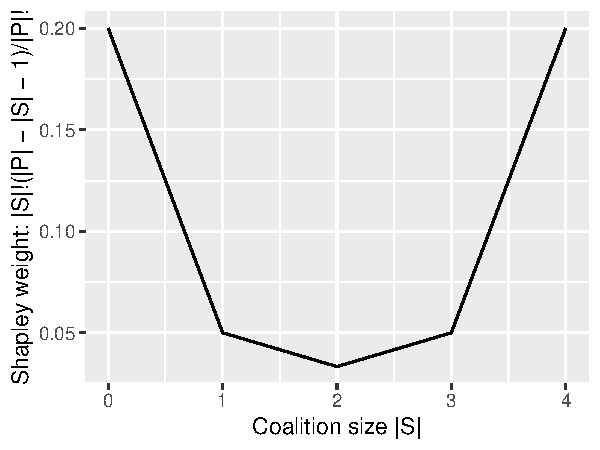
\includegraphics[width=0.5\textwidth]{figure/shapley-weights}
%       \end{center}
% \end{frame}

\begin{frame}{Bike Sharing Dataset}

\begin{center}
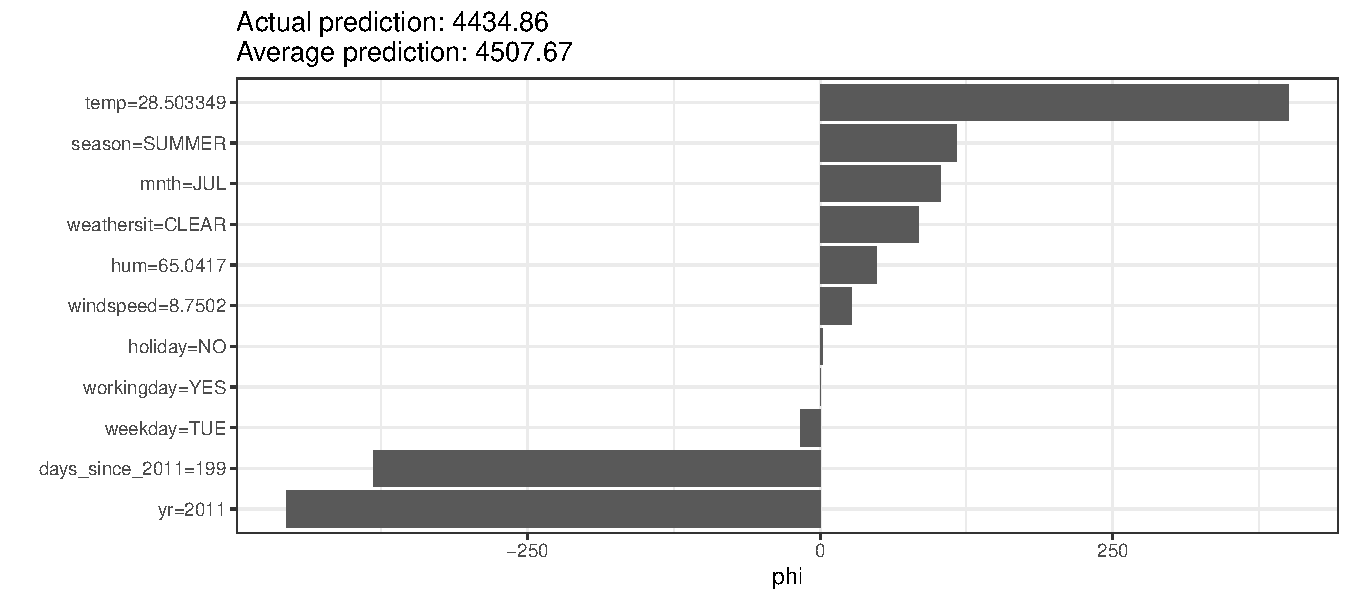
\includegraphics[width=0.6\textwidth]{figure/shapley-bike.pdf}%{figure_man/bike-sharing03.png}%
\end{center}

% \begin{itemize}
%     \item Shapley values of observation $i = 200$ from the bike sharing data
%     \item Difference between model prediction of this observation and the average prediction of the data is fairly distributed among the features (i.e., $4434 - 4507 \approx -73 $)
%     \item Feature value temp = 28.5 has the most positive effect, with a contribution (increase of prediction) of about +400
% \end{itemize}
\begin{itemize}%[<+->]
  \item Shapley decomposition for a single prediction in bike sharing dataset %(observation $i = 200$)
  \item Model prediction: $\fh(\xv^{(200)}) = \textbf{4434.86}$ vs. dataset average: $\E_\xv[\fh(\xv)] = \textbf{4507.67}$
  \item Total feature attribution: $\sum_j \phi_j = \textbf{-72.81}$\\
  $\leadsto$ Explain downward shift from mean prediction
  \item Temperature (with value $28.5^\circ$C) is the strongest positive contributor: $+400$
  \item Features \texttt{yr = 2011} and \texttt{days\_since\_2011 = 199} strongly reduce prediction\\
  $\leadsto$ Model captures lower bike demand in 2011 compared to 2012
\end{itemize}
\end{frame}


% \begin{frame}{Versions of the Shapley Value}

%   \begin{itemize}
%   \item KernelSHAP formulates the Shapley value solution as a regression problem using a specific kernel function. The authors show paralles to LIME and Deeplift.
%   \item TreeSHAP is a fast Shapley value computation method for tree-based models such as gradient boosted trees.
%  \end{itemize}
%     \tiny{Lundberg, Scott M., and Su-In Lee. "A Unified Approach to Interpreting Model Predictions." Advances in Neural Information Processing Systems 30 (2017): 4765-4774.}
%     \tiny{Lundberg, Scott M., Gabriel G. Erion, and Su-In Lee. "Consistent individualized feature attribution for tree ensembles." arXiv preprint arXiv:1802.03888 (2018).}
% \end{frame}

% \begin{frame}{ADVANTAGES AND DISADVANTAGES}
% 	\textbf{Advantages:}
% 	\begin{itemize}
% 	 \item \textbf{Solid theoretical foundation} in game theory
%         \item Prediction is \textbf{fairly distributed} among the feature values $\leadsto$ easy to interpret for a user
%         \item \textbf{Contrastive explanations} that compare the prediction with the average prediction
% 	\end{itemize}
% \vspace{0.25cm}
% 	\textbf{Disadvantages:}
% 	\begin{itemize}
% 		\item Without sampling, Shapley values need a lot of computing time to
% 		inspect all possible coalitions
% 		%\item The Shapley value of a feature value can be easily misinterpreted:
% 		%It is not the difference of the predicted value after removing the
% 		%feature from the model training; it is the contribution of a feature
% 		%value to the difference between the actual prediction and the mean
% 		%prediction, given the current set of features
% 		\item Like many other IML methods, Shapley values suffer from the
% 		inclusion of unrealistic data observations when features are correlated
% 	\end{itemize}
% \end{frame}

\begin{frame}{Advantages and Disadvantages}

\textbf{Advantages:}
\begin{itemize}%[<+->]
  \item \textbf{Strong theoretical foundation} from cooperative game theory
  \item \textbf{Fair attribution:} Prediction is additively distributed across features\\
  $\leadsto$ Easy to interpret for users
  \item \textbf{Contrastive explanations:} Quantify each feature's role in deviating from the average prediction
\end{itemize}

\vspace{0.3cm}

\textbf{Disadvantages:}
\begin{itemize}%[<+->]
  \item \textbf{Computational cost:} Exact computation scales factorially with feature count\\
  $\leadsto$  Without sampling, all $2^p$ coalitions (or $p!$ permutations) must be evaluated
  \item \textbf{Issue with correlated features:} Shapley values may evaluate the model on feature combinations that do not occur in the real data
\end{itemize}

\end{frame}


\endlecture
\end{document}
